\documentclass{article}
\usepackage[utf8]{inputenc}
\usepackage[T1]{fontenc}
\usepackage{geometry}
\geometry{a4paper}
\usepackage{helvet}
\renewcommand{\familydefault}{\sfdefault}
\title{A research report on the frequency of crime in society}
\author{By Abule Augustine Arumadri 215014379 15/U/2633/PS}
\date{}
\setlength{\topmargin}{-1cm}
\usepackage{graphicx}
\begin{document}
\maketitle
\tableofcontents
\section{Introduction}
Crime  has always been a cancer in civil society, dating way back since the dawn of civilization. 
Crime is a very broad term, loosely meaning an illegal act or activity that can be punishable by law. Crimes can be divided into four major categories, personal crimes, property crimes, inchoate crimes and statutory crimes.

Crime, if not closely watched and fought, can be the downfall of civilization. It takes social sensitization and participation in the fight against this vice, and so through this project, I aim at getting people's personal accounts of their experiences of crimes in society. This data is very vital in tailoring useful and effective sensitization points and topics that will result into actual reduction in crime.


\section{Methodology}
The system consists of two interconnected parts: a smartphone application ODK Collect \cite{key:2} that runs a data collection form, and an online aggregate
 server that receives the submitted data and compiles it in whatever format designed. 

This online data repository can then be mined in many ways possible to get a clearer understanding of the frequency of crime,
 what type of crime, most affected areas, most targeted gender, and much more categories in order to effectively sensitize the public, 
based on this data, and possibly reduce crime.

\begin{figure}[h!]
\centering
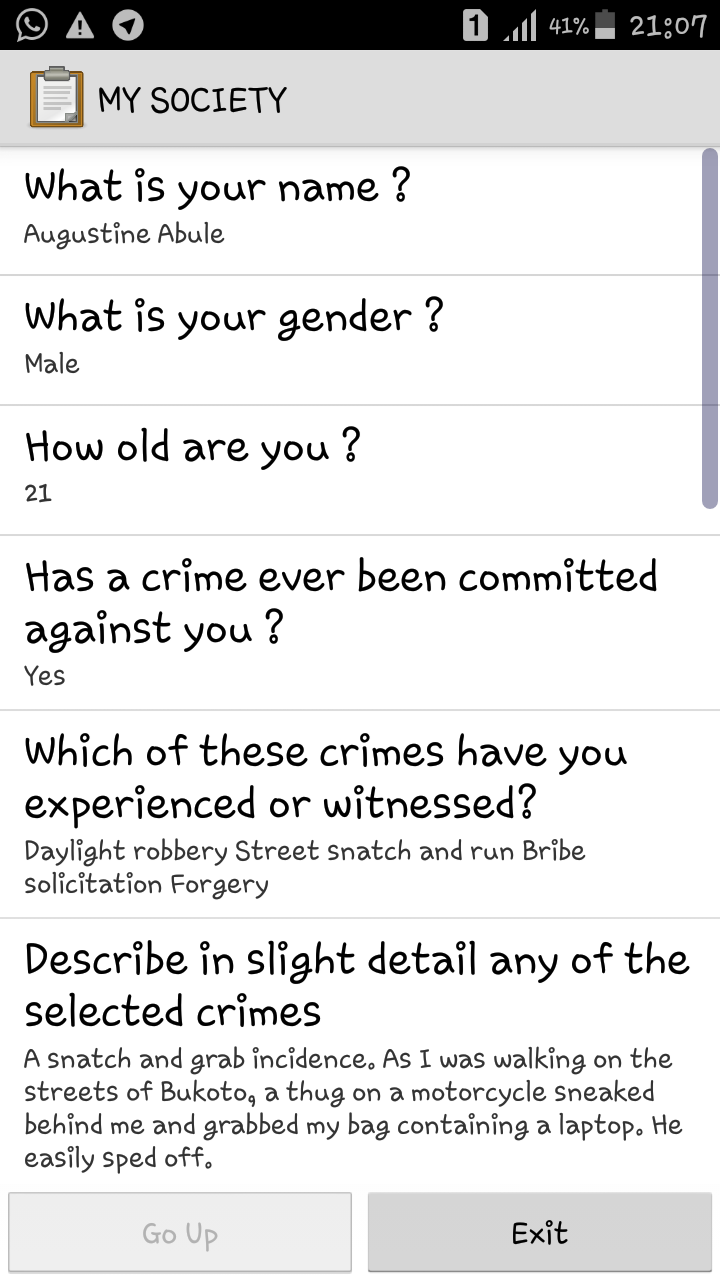
\includegraphics[width=1\textwidth]{Screenshot 1.png}
\end{figure}
\begin{figure}[h!]
\centering
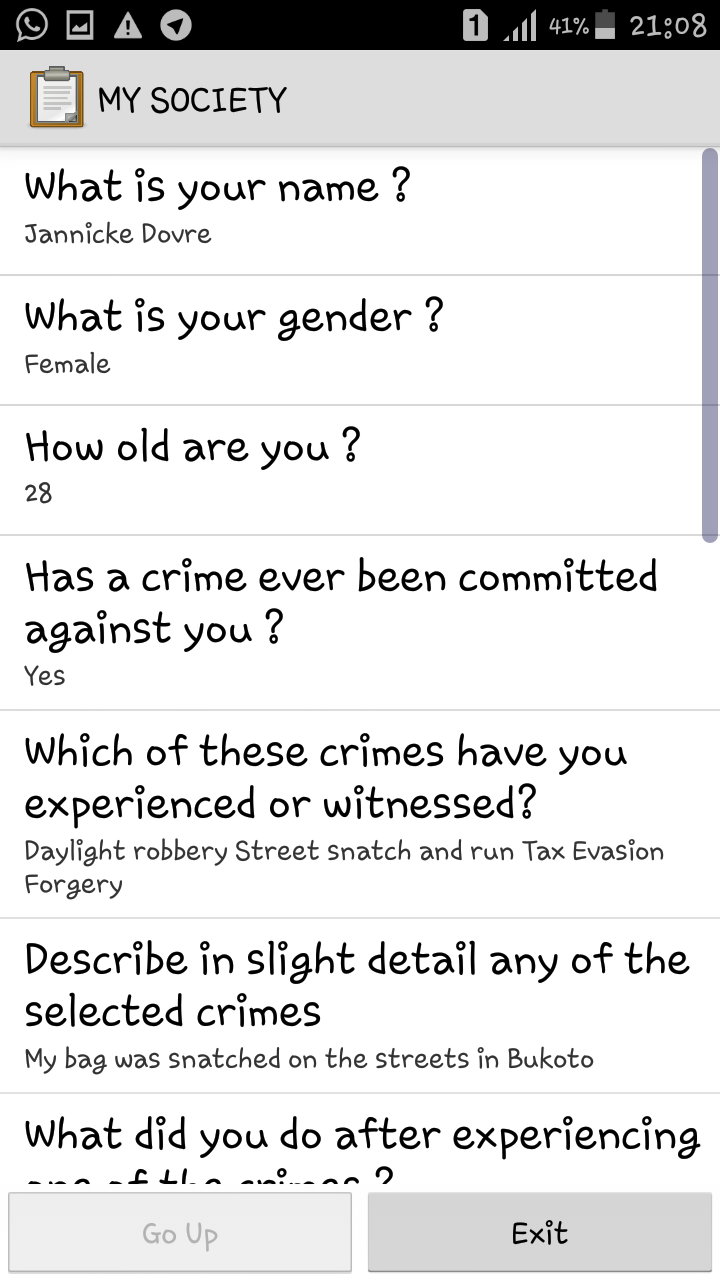
\includegraphics[width=1\textwidth]{Screenshot 2.png}
\end{figure}
\begin{figure}[h!]
\centering
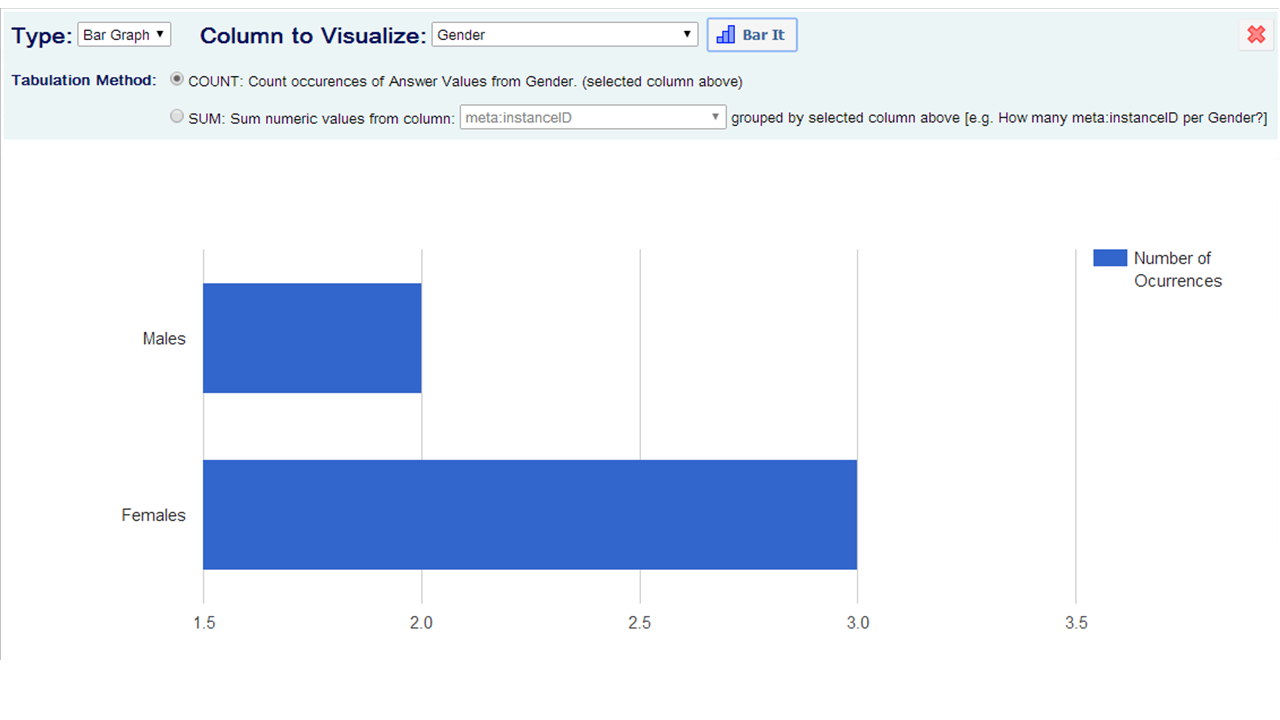
\includegraphics[width=1\textwidth]{Screenshot 3.png}
\end{figure}
\begin{figure}[h!]
\centering
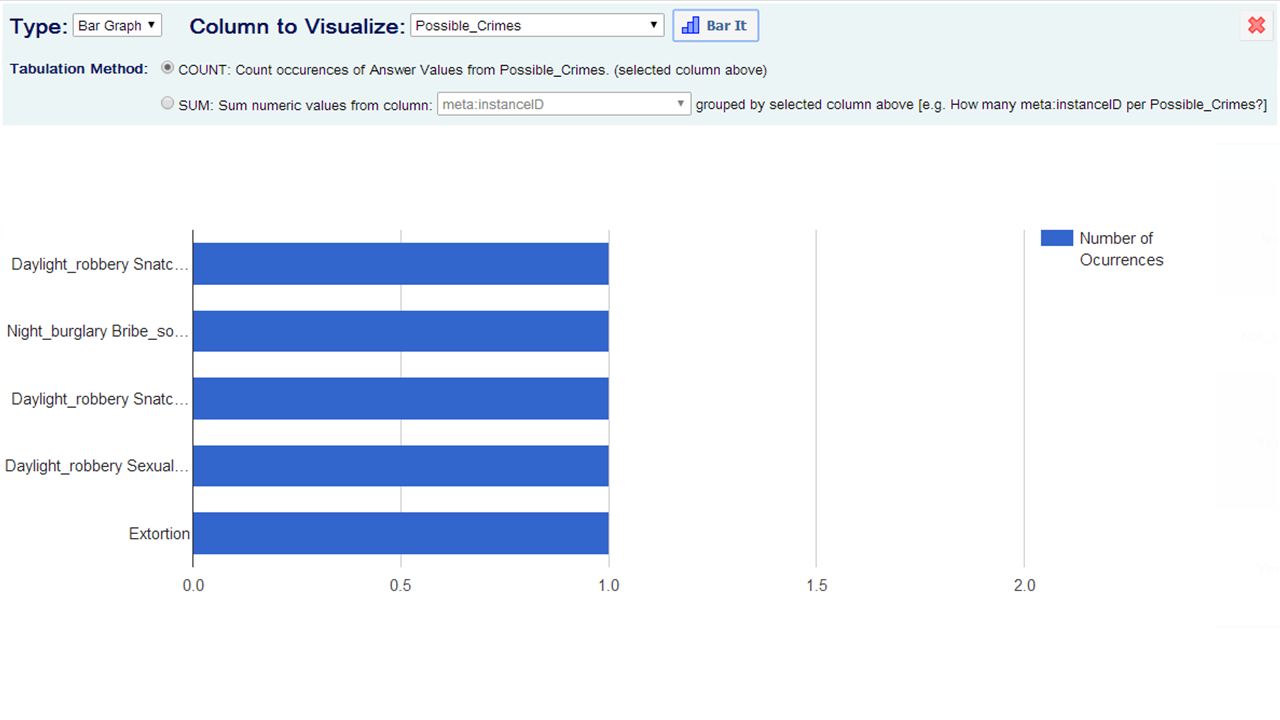
\includegraphics[width=1\textwidth]{Screenshot 4.png}
\end{figure}
\section{Results}
\begin{figure}[h!]
\centering
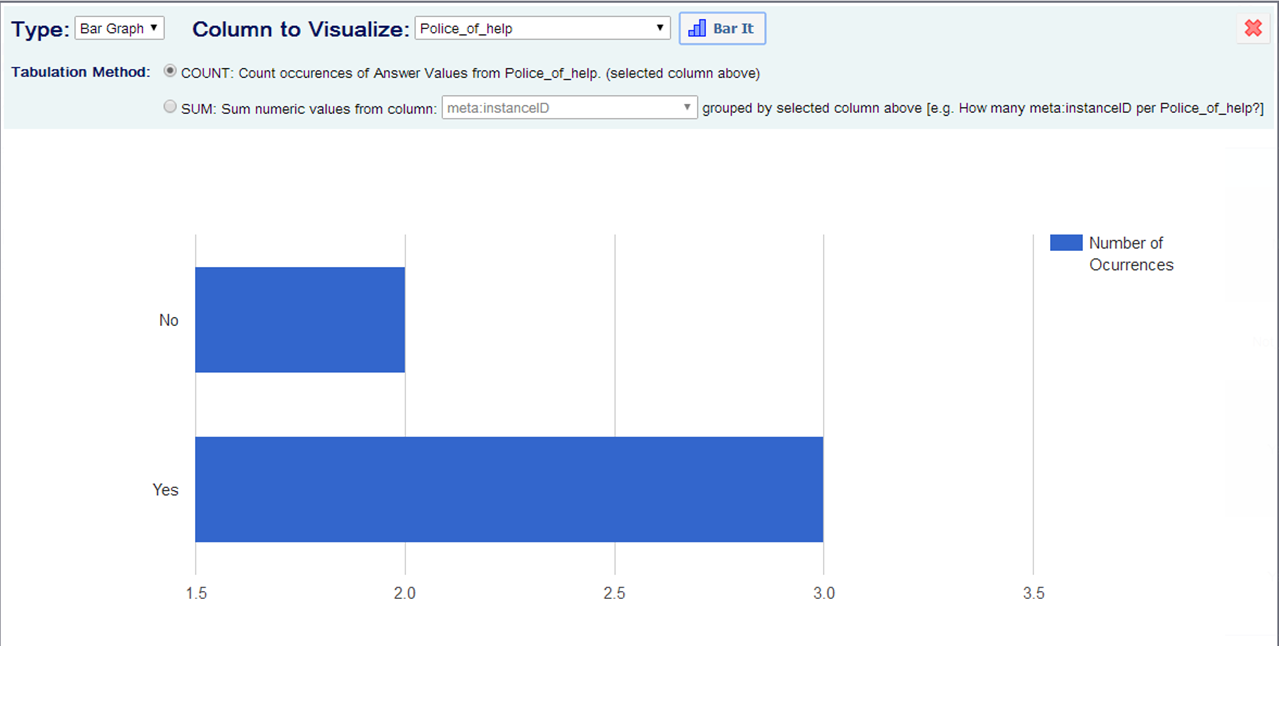
\includegraphics[width=1\textwidth]{Screenshot 5.png}
\end{figure}


\section{conclusion}

From the data received, and in comparison to police reports, it is indeed true that some crimes go unreported

\end{document}
